\documentclass[10pt, a4paper]{article}

% On écrit en français
\usepackage[utf8]{inputenc}
\usepackage[frenchb]{babel}
\usepackage[T1]{fontenc}

% Packages nécessaires
\usepackage{graphicx}
\usepackage{hyperref}

% Numérotation de page custom
\usepackage{fancyhdr}
\usepackage{lastpage}
\pagestyle{fancy}
\fancyhf{}
\rfoot{Page \thepage \hspace{1pt} sur \pageref{LastPage}}

% Police Helvetica <3
\usepackage{helvet}
\renewcommand*{\familydefault}{\sfdefault}

% Enlever les alinéas
\setlength{\parindent}{0pt}

% Marges plus larges pour faire moins LaTeX
\usepackage[left=3cm, right=3cm]{geometry}

% Sous titre de document
\usepackage{titling}
\newcommand{\subtitle}[1]{%
  \posttitle{%
    \par\end{center}
    \begin{center}\large#1\end{center}
    \vskip0.5em}%
}

% En tête complet de document
\newcommand{\Document}[1]{%
    \title{#1}
    \subtitle{Dématérialisation d'un processus de paiement}
    \author{
        COMETS Jean-Marie \\
        DELMARRE Adrian \\
        REYNOLDS Nicolas \\
        TURPIN Pierre
    }
    \date{\today}

    \maketitle \newpage

    \tableofcontents \newpage
}


\begin{document}

\Document{Plan d'assurance qualité}

\section{Présentation du plan d'assurance qualité}
\subsection{Présentation générale}
% TODO modifier cette section à chaque nouveau livrable
Ce document représente la version préliminaire du Plan d'Assurance Qualité
(PAQ). Il sera revu et complété au cours de la prestation des services
effectués. \\

En tant que version préliminaire, si des informations de ce document
contredisent des éléments d'un document d'expression du besoin ou de
présentation de solution, c'est ce dernier qui fait foi. \\

Le présent document s'applique aux prestations confiées par Aventix dans le
cadre du projet de conception \textit{"Dématérialisation d'un processus de
paiement"}. \\

\subsection{Objet du document}
Le PAQ est l'engagement de Aventix quant à la politique d'assurance qualité
applicable au projet.
Il rappelle également nos obligations envers Aventix sur le projet de conception.
\\

Le PAQ décrit :
\begin{itemize}
  \item La présentation générale du Plan d'Assurance Qualité.
  \item Les documents à livrer dans le cadre de ce projet de conception.
  \item La méthodologie applicable pour la réalisation des livrables.
  \item Le processus de gestion de la qualité.
  \item Le glossaire des principaux termes, expressions et abbréviations
    métiers utilisées
\end{itemize}

\section{Documents à livrer dans le cadre du projet de conception}
La liste des livrables brièvement décrite est fournie dans le document
d'initialisation du projet. \\

Voici un rappel des documents applicables :
\begin{itemize}
  \item Dossier d'initialisation
  \item Expression des besoins
  \item Étude comparative
  \item Architecture applicative
  \item Architecture technique
  \item Business plan
\end{itemize}

\subsection{Dossier d'initialisation}
Le dossier d'initialisation est un document rappelant le contexte et l'objet du
projet de conception suivi. \\

Ce dernier établit également la liste des livrables ainsi qu'une description
schématisée et textuelle de l'organisation de l'équipe dans la gestion des
tâches. \\
Enfin, une analyse de risques simplifiée est faite pour évaluer la cohérence du
projet. \\

Le dossier d'initialisation rappelera les points suivants :
\begin{description}
  \item[Contexte et objet du projet] Rappel du contexte du projet, de
    l'entreprise, le milieu dans lequel elle évolue, les concurrents.
    Solutions envisagées pour répondre aux besoins (expression des besoins
    très courte).
  \item[Description des livrables] Chaque livrable avec une description courte
    de son contenu.
  \item[Gestion des tâches] Fonctionnement des tâches et gestion de l'équipe au
    sein du projet.
  \item[Organisation de l'équipe] Listing des membres de l'équipe et de leur
    qualification.
  \item[Analyse des risques] Analyse des risques aux sein du projet (gestion
    projet, livrable, contenu, retard, respect des attentes, respect de
    la charte, du fonctionnement, qualité).
\end{description}

\subsection{Étude comparative (Benchmarking)}
Ce document est un comparaison de la solution envisagée par rapport aux autres
solutions de paiements et leur interconnexion avec un SI. \\

Celle-ci est présentée comme une synthèse bibliographique et devra citer ses
sources à la fin du rapport afin de justifier les choix effectués. \\

Chaque solutions proposées doit disposer d'une étude de ses points forts et ses
points faibles. \\

La synthèse n'indique pas de solutions choisies dans l'étude technique mais
seulement une comparaison des différents cas. Le choix de la ou les bonnes
solutions sera effectué dans l'établissement de l'architecture applicatif et
technique. \\

L'étude comparative s'effectuera sur les deux points suivants :
\begin{enumerate}
  \item Bornes des paiements (lecteur cartes, NFC, RFID, ...)
  \item Communication entre un SI et une banque via EDI
\end{enumerate}

\subsection{Expression des besoins}
L'expression des besoins est une étude préliminaire sur laquelle notre étude
technique va se baser. Il n'y aura pas d'étude de besoins postérieure prenant en
compte les résultats et solutions finales. \\

L'étude reprend les points suivants :
\begin{enumerate}
  \item Rappel contextuel de la conception
  \item Description des objectifs du projet
  \item Présentation des spécifications fonctionnelles
    \begin{enumerate}
      \item Listing des acteurs
      \item Analyse des besoins fonctionnels
      \item Expression des utilisations
    \end{enumerate}
\end{enumerate}

\subsubsection{Rappel contextuel de la conception}
Cette partie reprend le contexte externe et interne du projet de conception. \\

Aucun schéma n'est à fournir et seul un simple récapitulatif suffit. \\

\subsubsection{Description des objectifs du projet}
Cette description reprend les objectifs à faire pour satisfaire les besoins du
client. \\

Chacune des demandes de Aventix est répertoriées précisément une par une sous
forme d'une liste à puce. Les contraintes sont également listées clairement. \\

Cette partie permet de montrer notre compréhension du problème d'Aventix et de
spécifier si des attentes sont hors du périmètre de l'étude. \\

\subsubsection{Présentation des spécifications fonctionnelles}
\paragraph{Listing des acteurs}
~\\
Cette partie spécifie l'ensemble des acteurs utilisés dans l'étude de conception. \\

L'ensemble est présenté sous la forme d'une liste reprenant le nom de l'acteur
utilisé lié à une description de ce qu'il fait. \\

\paragraph{Analyse des besoins fonctionnels}
~\\
L'analyse des besoins propose une énumération claire et précise sous forme de
listes hiérarchisées des différentes attentes identifiées. \\

\paragraph{Expression des utilisations}
~\\
Les utilisations du produit sont recensées dans cette partie et doit
correspondre à une description détaillée de chaque analyse de besoins
fonctionnels spécifiée dans la partie précédente. \\

L'architecture globale de le communication dans le système est représenté
d'abord par un MCC (Modèle Conceptuel de la communication). \\

Chaque besoins fonctionnels est alors détaillée par un MOT (Modèle
Organisationnel de Traitements). Dans le cas ou le MOT est trop simple, une
courte description textuelle est mise à la place. \\

Les MOT devront suivre le modèle de la figure \ref{fig:mot-skeleton}. Ce schéma
n'est pas exhaustif sur toutes les formes possibles mais permet d'avoir un
squelette de développement de ces modèles organisationnels. \\

\begin{figure}[ht]
    \centering
    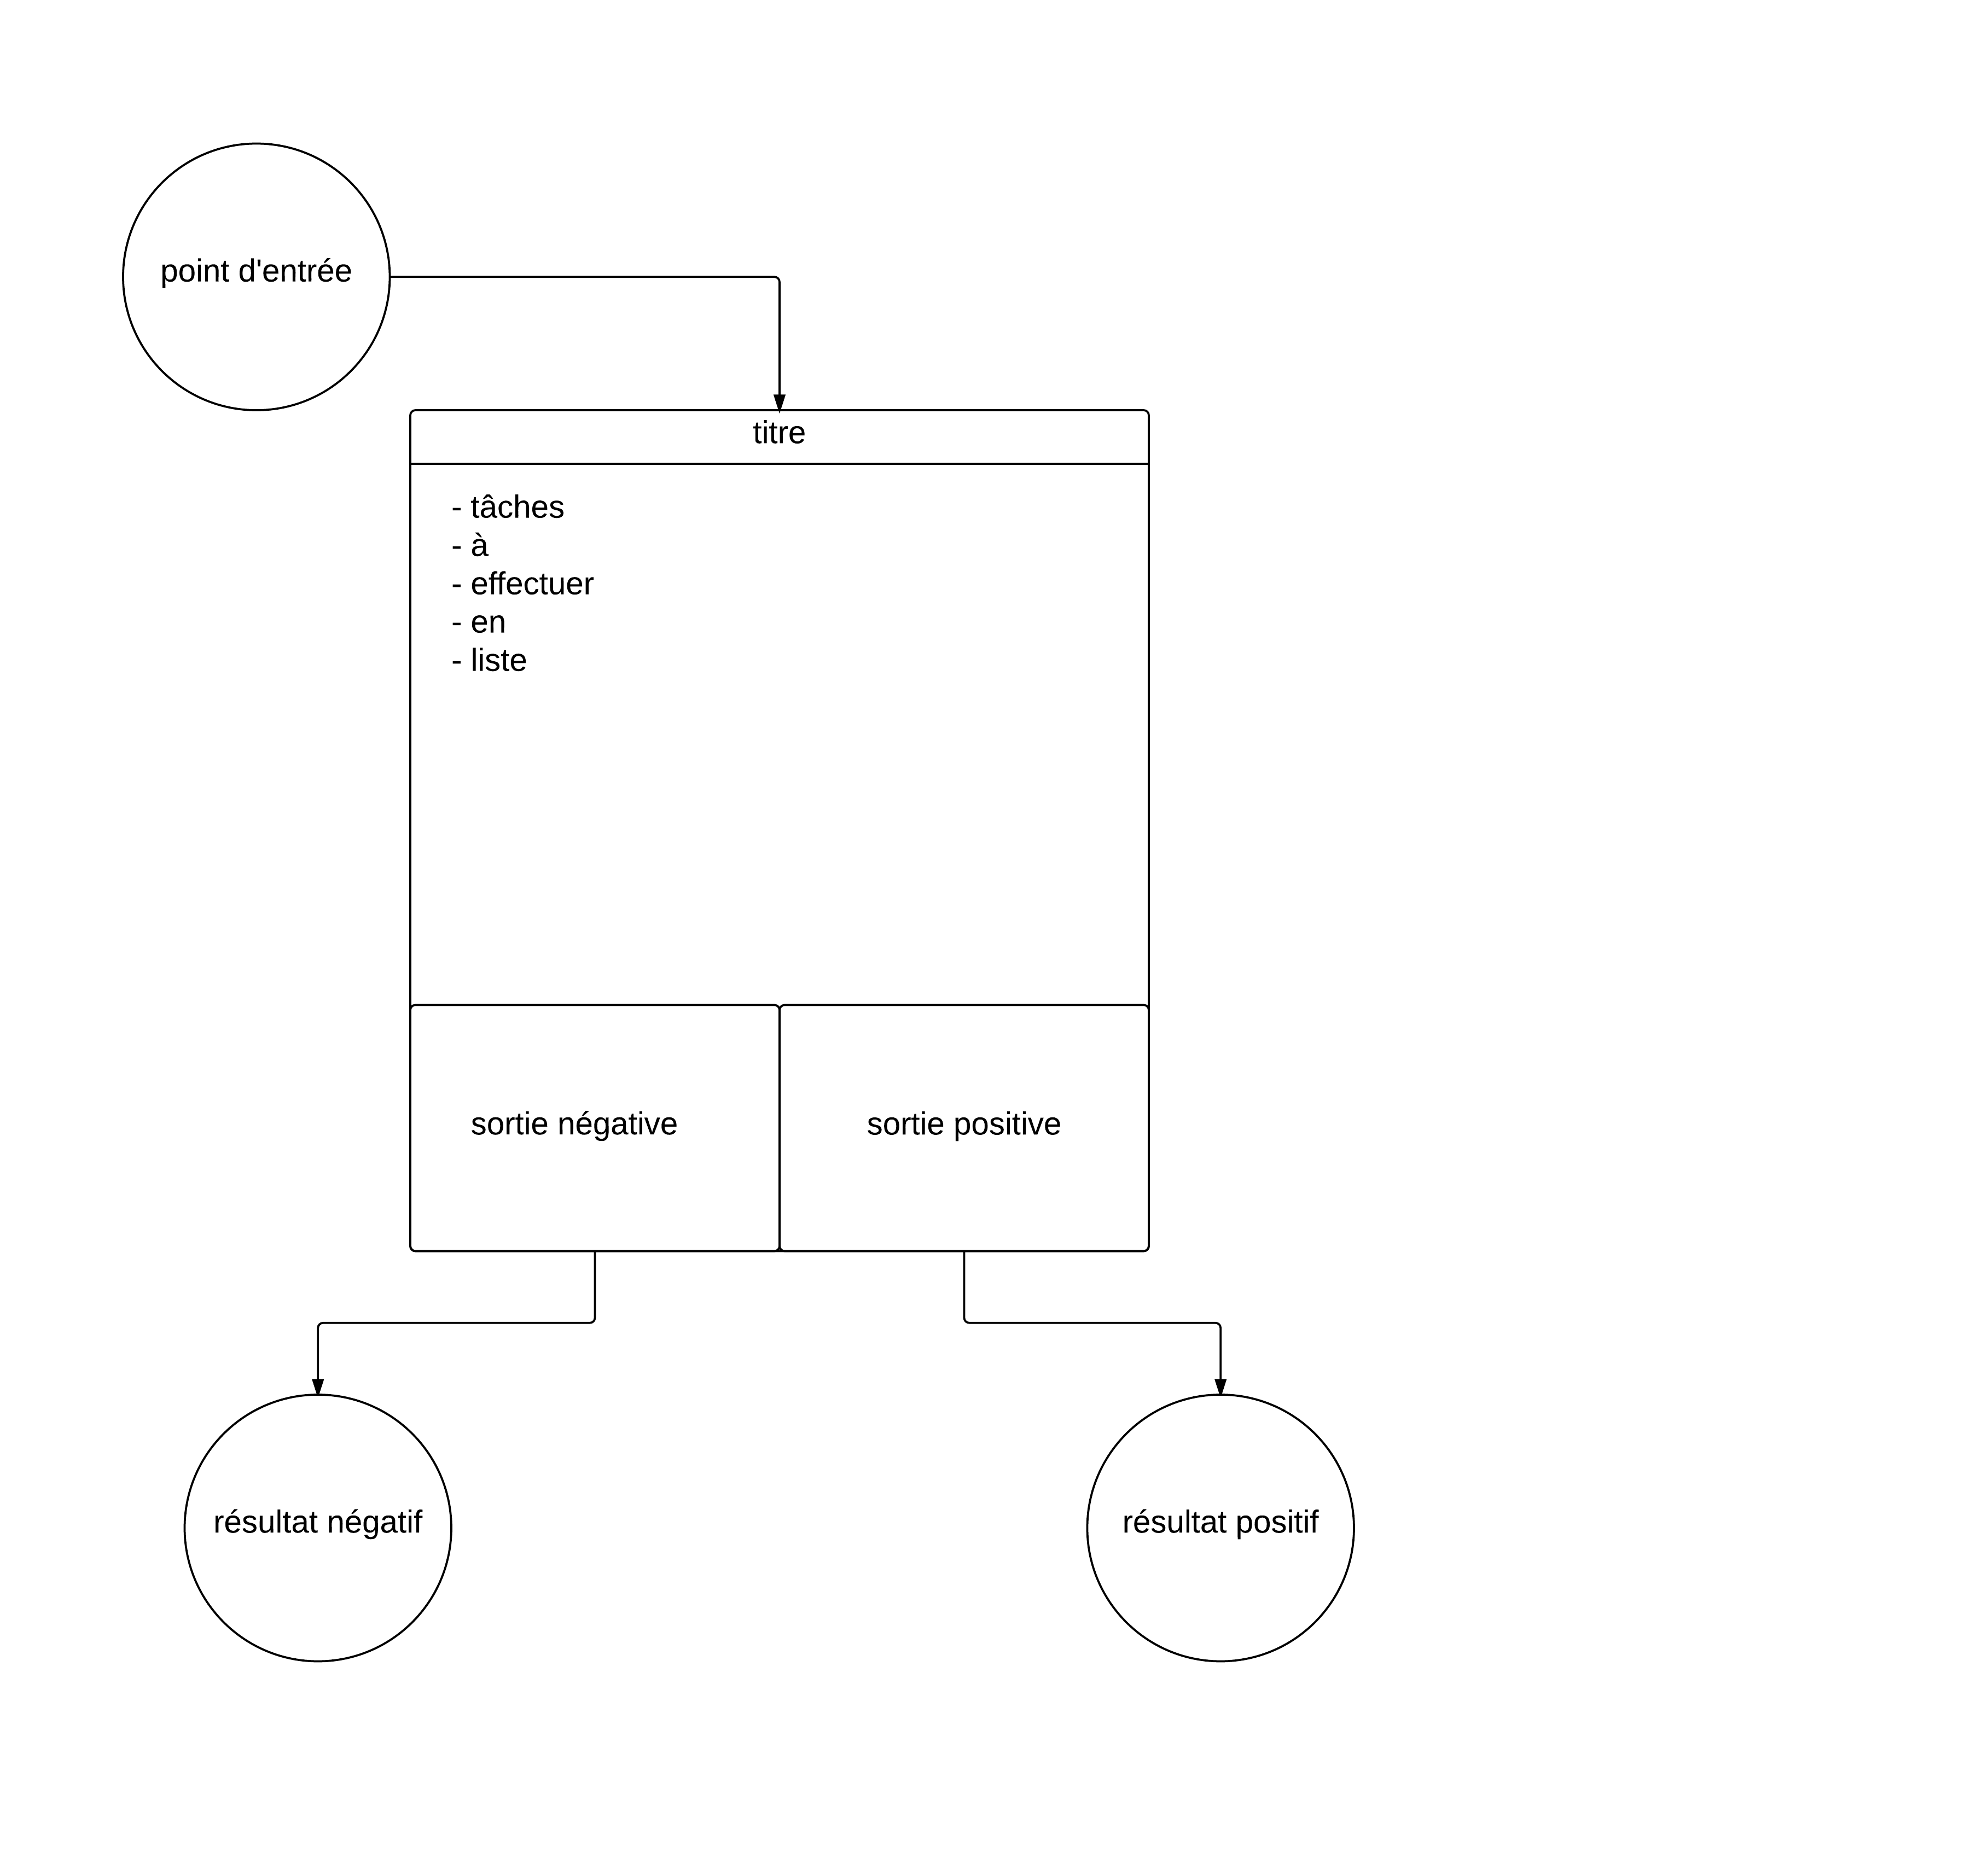
\includegraphics[width=\textwidth]{mot-skeleton}
    \caption{Squelette des Modèles Organisationnels de Traitements (MOT)}
    \label{fig:mot-skeleton}
\end{figure}

\subsection{Architecture Applicative}
MCD global du système
Définition des blocs fonctionnels
Liste des applications
Services applicatifs
Utilisation des services (forme à définir)
% TODO remplir cette section

\subsection{Architecture Technique}
\begin{enumerate}
  \item Stockage
  \item Recherche
  \item Consultation
  \item Communication avec les partenaires et les employés
  \item Sécurité
  \item Disponibilité 24/24 7/7
  \item Création de services métiers facile
  \item SI évolutif et maintenable
  \item (Privilégier les offres cloud computing orienté service SOA)
\end{enumerate}

\subsection{Business plan}
\begin{enumerate}
  \item Produit service
  \item Étude du marché
  \item Plan marketing
  \item Plan d'opération
  \item Stratégie de sortie
  \item Évaluation des couts
  \item Analyse des risques
\end{enumerate}

\section{Méthodologie de réalisation}
\subsection{Réunion de travail}
Afin d'avoir un comportement agile dans l'élaboration des prestations, l'équipe
entière doit se réunir au moins une fois par semaine. Cette réunion permet à
chacun d'échanger son avancée aux autres afin de vérifier et de corriger le
planning prévisionnel établi pour le projet. \\

Cette agilité de travail nous permet d'établir une politique d'organisation
scrum. La gestion de projet se fait donc plus facilement en découpant les
travaux à effectuer en \textit{sprints} dynamiques qui peuvent être modifiés
d'une réunion à une autre afin réagir à une situation de retard, voire d'avance
de la prestation. \\

Un face-à-face hebdomadaire est également prévu avec le prestataire Aventix.
Cela permettra de démontrer notre engagement et la qualité de la prestation
tout en recevant un retour direct pour clarifier l'expression des besoins et
l'établissement d'une solution technique ainsi qu'un business plan. \\

\subsection{Maîtrise des livrables}
\subsubsection{Format des livrables}
La forme de tous les documents est globalement régie par un guide de style que
nous avons spécifié en interne. \\
Ce dernier n'est pas disponible en livrable pour Aventix. \\

Dans le cas où un document impose des règles de forme particulière telles que
des schémas, des illustrations, ..., ces dernières sont disponibles et
spécifiées précédemment dans la présentation des livrables. \\

Également dans les spécification des présentations des livrables, la forme et
le structure de ceux-ci est fourni. Cela permet d'avoir des règles de
structures détaillées, complètes et centralisées. La cohésion et l'intégrité du
travail produit et alors certifié. \\

\subsubsection{Remise des livrables}
La remise des livrables au client Aventix se fera au fur et à mesure de l'étude
de la conception. \\

Le \textbf{mercredi 15 octobre 2014}, le dossier d'initialisation sera transmis.
Une étude comparative sur les lecteurs de cartes à puce et leur interconnexion
avec un système d'information sera également donnée pour établir et justifier
notre choix de conception sur les architectures applicative et technique
choisies. \\
L'expression des besoins sera également fournis. \\

Le \textbf{mercredi 22 octobre 2014}, le dossier d'architecture applicative sera rendu
et validé. \\

Le \textbf{mercredi 5 novembre 2014}, le dossier d'architecture technique sera délivré.
Un document expliquant la solution EDI choisie pour l'échange avec la banque
sera également remis. \\

Le business plan sera donné au plus tard le \textbf{mercredi 19 novembre 2014}. \\

Une revue finale avec Aventix sera dispensée entre le \textbf{mercredi 5
  novembre} et le \textbf{mercredi 19 novembre} 2014 sur rendez-vous et accord
des deux parties.  Cette réunion d'explication nous permettra d'expliquer la
démarche effectué et la solution choisie durant la prestation afin d'améliorer
la prise en main du business plan et d'assurer la qualité des directives
métiers de la part d'Aventix. \\

\subsection{Maîtrise des risques}
Les méthodologies assure une bonne maîtrise des différents risques possible
durant l'étude du projet de conception. \\

En effet, l'organisation de travail agile permet de correctement prévenir les
risques d'écart du planning prévisionnel. Comme ce dernier est dynamique et
peut être ajusté à chaque itération, le rythme de travail peut être modifié
afin de s'en rapprocher le plus. Cela est valable pour les retards mais
également pour les surplus de travail. \\

Les revues et validations régulières de la part d'Aventix permettent d'avoir un
retour d'approbation et de contentement, limitant les risques de non
satisfaction de la prestation fournie. \\

Enfin, le simple suivi des règles de gestion de la qualité de ce document, qui
sont approuvées par Aventix, empêchent tomber dans le cas du paragraphe
précédent. \\

\section{Gestion de la qualité}
La gestion de la qualité de la prestation est assurée par un suivi systématique
de ce document ainsi que grâce à la méthodologie de travail de l'équipe. \\

De plus, le processus d'écriture des livrables requiert la relecture par le
responsable qualité de l'équipe. Cette phase de correction permet, en plus
d'avoir un document propre, de gérer correctement la cohérence entre les
différents documents. \\

Les termes métiers utilisés dans les documents sont alors répertoriés dans le
glossaire et unifiés à travers tous les documents. \\
Également les documents doivent remplir les conditions de qualité attendu
spécifié dans ce document. \\

Dans le cas d'un non-respect grave des attentes, le document est redistribué à
l'auteur pour amélioration pour repasser ensuite par une phase de relecture et
correction. \\
Sinon, le document est renvoyé à l'auteur afin qu'il approuve les modifications
pour valider définitivement le document. \\

Dans le cas où un travail requiert des attentes techniques spécifiques, un de
nos expert peut faire partie du processus de correction afin de certifier la
qualité des livrables finaux. \\

\section{Glossaire}

\begin{description}
  \item[Carte à puce] Objet possédant un identifié et pouvant être connecté par
    un lecteur de carte à puce.
  \item[Lecteur de carte à puce] Lecteur pouvant lire des cartes à puce par un
    protocole défini.
  \item[Borne NFC] Lecteur de cartes à puce NFC installé chez un commerçant et qui
    permet de transmettre les données relatives à une transaction commerciale.
  \item[Entreprise] Personne légale représentant une entreprise devant la loi.
  \item[Commerçant] Entreprise dont une des activités concerne la vente de
    biens pouvant être achetés par une solution de titre restaurant.
  \item[Commande] Demande d'une quantité de carte à puce par une entreprise.
  \item[Facture] Note précisant les prix, la quantité et la nature des
    marchandises ou services vendus. Par défaut on désignera la note de
    paiement d'une commande d'une entreprise.
  \item[Document de prospection] Document présentant la solution ci-présente,
    en vue de démarcher des commerçants, des entreprises ou encore des
    utilisateurs. Plusieurs versions de ce document existeront, selon la cible
    de la prospection.
  \item[Client direct] Désigne soit une entreprise, soit un commerçant.
  \item[Utilisateur final] Utilisateur de la carte à puce.
  \item[Banque] Enseignes bancaires garantissant la sécurité des transactions
    (terminaux et internet) et leurs échéances.
  \item[Installateur mainteneur] Artisans accrédités responsables de la mise en
    place des lecteurs de cartes à puce chez les commerçants partenaires, ainsi
    que des opérations de maintenance.
  \item[Fournisseur] Entreprises fabricant ou important les lecteurs de cartes
    à puce mises en place chez les commerçants partenaires.
  \item[Service marketing] Service responsable de la prospection de nouveaux
    clients, quelle que soit leur nature, du dimensionnement (nombre de bornes,
    etc.) et de l’établissement de contrats.
  \item[Service commande] Poste de travail qui traite les commandes (saisie,
    édition et envoi de bons de commande). Cet acteur s’occupe également des
    devis.
  \item[Service facturation] Poste de travail qui traite les factures
    (élaboration des règles de facturation, édition et ennvoi des factures).
    Cet acteur s’occupe également des expéditions de puces NFC à destination
    des entreprises.
  \item[Service traitement] Service chargé de surveiller le traitement des
    transactions. Une transaction s’effectue entre un commerçant et le système.
    Ce service est également chargé de mettre à jour les données suite aux
    sollicitations des employeurs ou des employés.
  \item[Service client] Interface entre les clients (entreprises
    et commerçants), garant de la qualité des services proposés et récipendaire
    des réclamations éventuelles.
\end{description}

\end{document}

% vim: ft=tex et sw=2 sts=2
